\chapter{Discussion}

\section{Quantitative analysis}


\textbf{Test for synonyms...} on machine learning and language model to be done
\begin{figure}[h!]
    \centering
    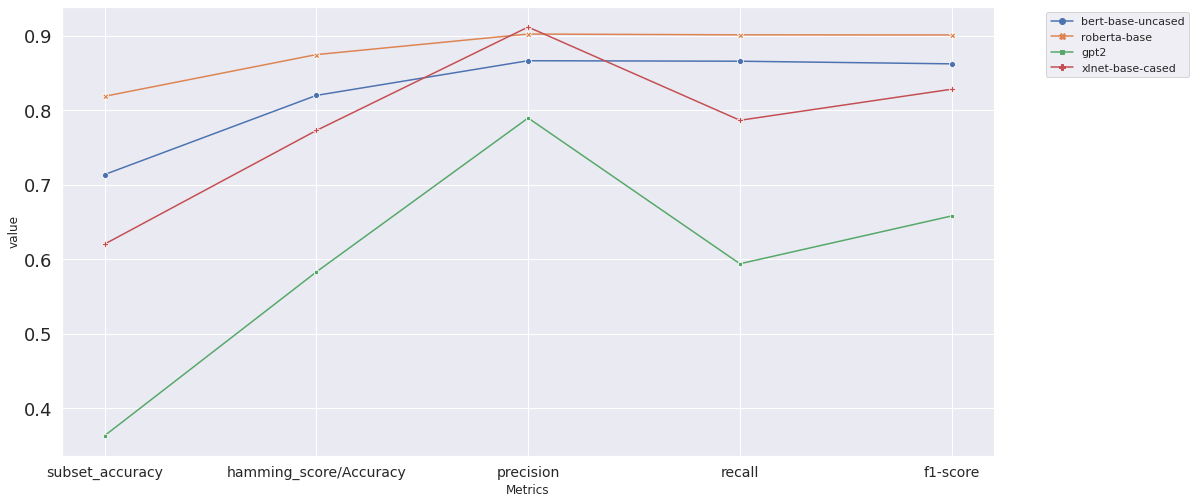
\includegraphics[width=1\textwidth]{thesis/figures/summary.png}
    \caption{Sample average metrics summary results of language models }
    \label{fig:model_wise_group_LM}
\end{figure}
\subsection{Evaluation of Language models}
% \begin{figure}[h!]
%     \centering
%     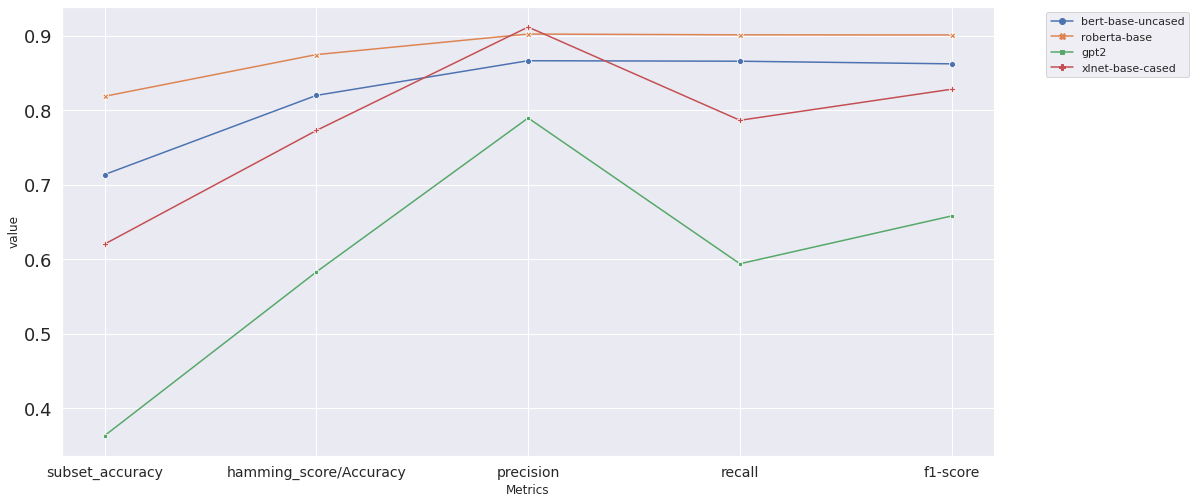
\includegraphics[width=1\textwidth]{thesis/figures/summary.png}
%     \caption{Sample average metrics summary results of language models }
%     \label{fig:model_wise_group_LM}
% \end{figure}
% \begin{figure}[h!]
%     \centering
%     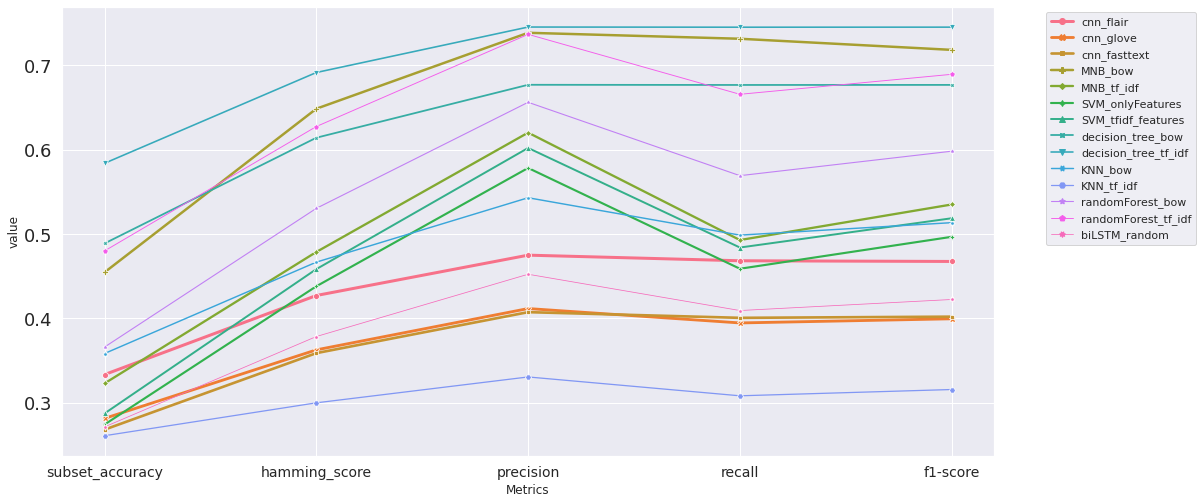
\includegraphics[width=1\textwidth]{thesis/figures/Baslines.png}
%     \caption{Sample average metrics summary results of language models }
%     \label{fig:model_wise_group_LM}
% \end{figure}
\begin{itemize}
    \item Roberta: The advantages of using transfer learning and language models is the robustness of the model apart from the effectiveness.
\end{itemize}
\subsection{Evaluation of Baselines}
\begin{figure}[h!]
    \centering
    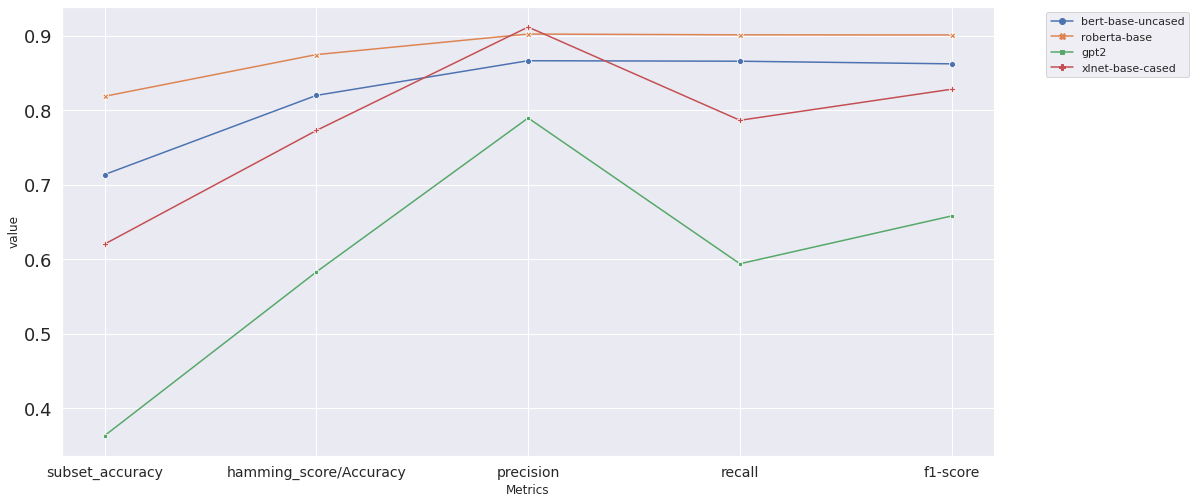
\includegraphics[width=1\textwidth]{thesis/figures/summary.png}
    \caption{Sample average metrics summary results of language models }
    \label{fig:model_wise_group_LM}
\end{figure}
\begin{figure}[h!]
    \centering
    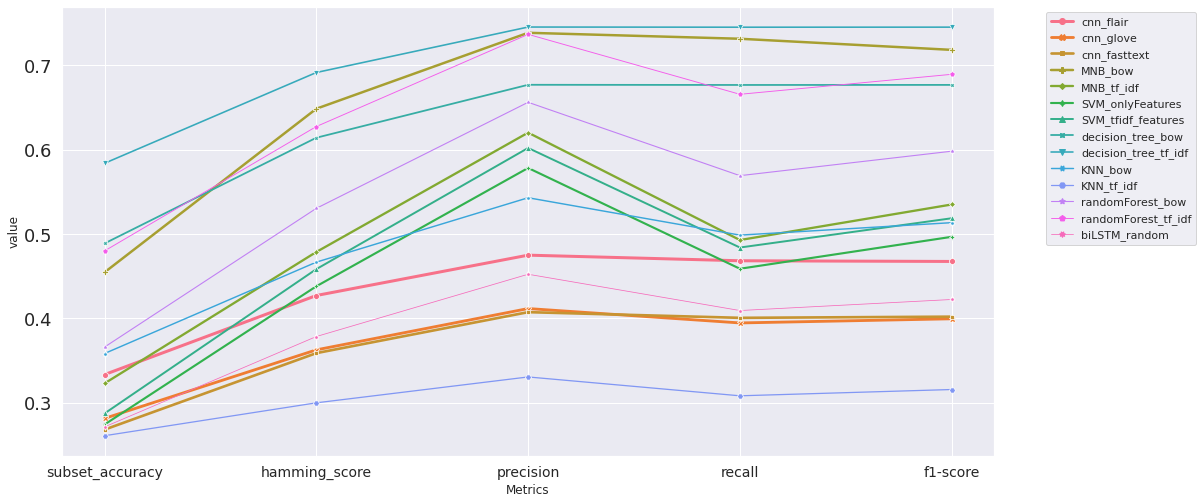
\includegraphics[width=1\textwidth]{thesis/figures/Baslines.png}
    \caption{Sample average metrics summary results of language models }
    \label{fig:model_wise_group_LM}
\end{figure}
\begin{itemize}
    \item MNB and decision tree: Through training these models is far cost-effective, the robustness of the model remains an issue. 
    \item The results on the test set states that these machine learning models are performing well on explicit features, but when tested with random samples, it might fail miserably. 
\end{itemize}


\section{Qualitative analysis}
\begin{itemize}
    \item Interpretation of results and Selecting best performing model 
    \item Best performing model discussion with manual sentences (Test cases ) 
    \begin{itemize}
        \item Effectiveness (Metrics)
        \item Efficiency (time)
        \item Test Explicit(Associations to stereo attribute) and implicit (Analogies) stereotypes
        \begin{itemize}
            \item Explicit stereotypes : Overt expression of target with attribute, e.g. target : African, stereotypic attribute : good at running
            \item Implicit stereotypes : Subtle expression of stereotypes where the target is an instance of target and where the attribute may be synonymous as well
            e.g. Target : African name, stereotypic attribute :  good at running 
        \end{itemize} 
        \item Test for explicit stereotypical bias statements  (stereotypical, anti-stereotypical and unrelated)
        \item Test by changing target other than the provided in dataset 
        \item Manual evaluation with respect to selected arguments (IBM dataset) and analysis with respect to user study 
    \end{itemize}
\end{itemize}